%++++++++++++++++++++++++++++++++++++++++
% Don't modify this section unless you know what you're doing!
\documentclass[letterpaper,12pt]{article}
\usepackage{tabularx} % extra features for tabular environment
\usepackage{amsmath}  % improve math presentation
\usepackage{graphicx} % takes care of graphic including machinery
\usepackage{siunitx}
\usepackage[margin=1in,letterpaper]{geometry} % decreases margins
\usepackage{cite} % takes care of citations
\usepackage[final]{hyperref} % adds hyper links inside the generated pdf file
\usepackage{caption}
\captionsetup[table]{skip=10pt}
\usepackage{float}
\usepackage{indentfirst}
\hypersetup{
	colorlinks=true,       % false: boxed links; true: colored links
	linkcolor=blue,        % color of internal links
	citecolor=blue,        % color of links to bibliography
	filecolor=magenta,     % color of file links
	urlcolor=blue         
}
%++++++++++++++++++++++++++++++++++++++++

\begin{document}

\title{Exploration of Hyperfine Splitting in Fe-57 Using Mössbauer Spectroscopy}
\author{Z. \AE ther, W. Lucas, H. William}
\date{\today}
\maketitle


\begin{abstract}
Using Mössbauer Spectroscopy, we measured the hyperfine splitting effect of the Fe-57 isotope. We mapped the resonant spectrum of transition energies, and we conclude that the magnetic moment of the first excited state of Fe57 is $\mu_{1/2}=4.86*10^{-13}$ eV/G with an error of $\pm5*10^{-15}$ eV and the size of the internal magnetic field is 314 kG with an error of 3 kG. Our measurement of $\mu_{1/2}$ is consistent with theoretical expectation. 
\end{abstract}

\pagebreak




\section{Introduction}

A physical exploration of hyperfine splitting effects may be helpful to better understand the measurable results of quantum mechanics. Although mathematical derivation of physical quantities is generally more precise, a contradicting physical measurement can be a blinding revelation. Accurate measurement is crucial for physicists to confirm their mathematical theories, and in this case, to prove the existence of quantum hyperfine phenomena. Mössbauer Spectroscopy is a method of precisely measuring the hyperfine splitting effect, and can be used to explore these effects with measurable precision.\


\subsection{Mössbauer Spectroscopy}

    When gamma rays incident on the absorber are of equal energy to the transition energies of the absorber, the photon is absorbed. There is recoil energy described by \

    \begin{eqnarray}
        R = (E_0)^2/ (2Mc^2) \label{eqn:recoil}\,,
    \end{eqnarray}

    associated with absorption in the nucleus. However, in a lattice structure, recoil energy causes vibration known as a phonon. Because a single absorption event is not enough to excite a phonon, no gamma energy is lost to the recoil of the absorbing molecule. This provides an extremely resolute spectrum of energy. The phenomenon of recoilless absorption is known as the Mössbauer Effect. 


\subsection{Hyperfine Splitting}

    The protons in the nucleus of Fe-57 have a magnetic dipole moment which creates a magnetic field. In the presence of this field, the energy levels of the atom are split relative to the unsplit energy by an amount (see figure~\ref{fig:elevels})

    \begin{eqnarray}
        E = \mu Hm_{j}/I \label{eqn:split}\,,
    \end{eqnarray}

    \begin{figure}[ht] 
        \centering 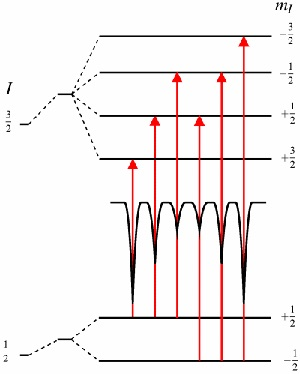
\includegraphics[scale=0.65]{hyperfine levels.jpeg}
        \caption{
                \label{fig:elevels}
                Energy level splitting for first excited state (I=3/2) and ground state (I=1/2)
        }
    \end{figure}

    Without considering splitting, the transition from the first excited state (I = 3/2) to the ground state (I = 1/2) is $E_0$=14.4 keV. When you take the split energies into consideration, this transition differs in energy from $E_0$ by an amount $\Delta E$.


\subsection{Doppler Effect}

    Mössbauer Spectroscopy utilizes the Doppler effect to parse through a small range of gamma ray energies. By constantly accelerating a gamma source, photons are released at different velocities relative to an absorber. These gamma rays will be received with different energies according to:

    \begin{eqnarray}
        \Delta E_{\mathrm{doppler}} = vE_{0}/c \label{eqn:doppler}\,,
    \end{eqnarray}

    where $E_{0}$ = 14.4 keV is the energy of the emitted photon. When this energy is equal to the shifts in transition energy due to hyperfine splitting, the absorption is resonant, corresponding to the valleys~(peaks) in the MCA.




\section{Experimental Methods}

The experimental setup we used to map the hyperfine splitting effects involved a Constant Acceleration Drive(CAD), a Fe-57 enriched absorber, a Geiger Muller tube, and a Multi Channel Analyzer(MCA). 

\begin{figure}[ht] 
        \centering 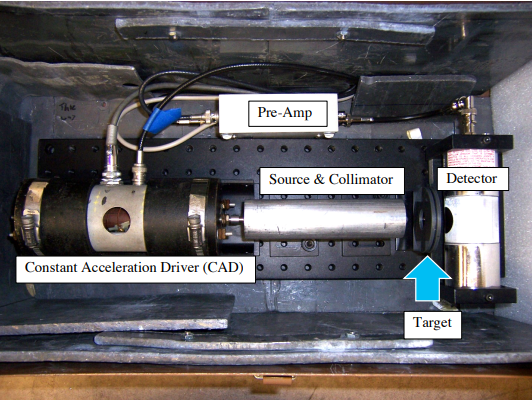
\includegraphics[scale=0.5]{Setup.png}
        \caption{
                \label{fig:setup}
                Setup of the Mössbauer Spectroscopy experiment
        }
\end{figure}  

The Co-57 source is mounted inside the CAD (Fig.~\ref{fig:setup}), to be oscillated at constant acceleration. The Fe-57 absorber is mounted upon the target (Fig.~\ref{fig:setup}) in line with the source, and in front of the Geiger Muller detector (Fig.~\ref{fig:setup}). Gamma rays incident on the recoilless absorber pass through towards the detector, unless absorbed. Pulses from detector, indicating counts, are analyzed and displayed on the MCA via the UCS-30 software. 


\subsection{Energy Range Discrimination}

    To accurately measure the hyperfine splitting effects on the Fe57 nucleus, we needed to be sure that we were detecting only the 14.4 KeV gamma emission from the source. To do this, we conducted a preliminary test of the setup without the absorber. With the MCA in Pulse Height Analysis mode, we detected all of the cobalt emissions. 

    \begin{figure}[ht] 
        \centering 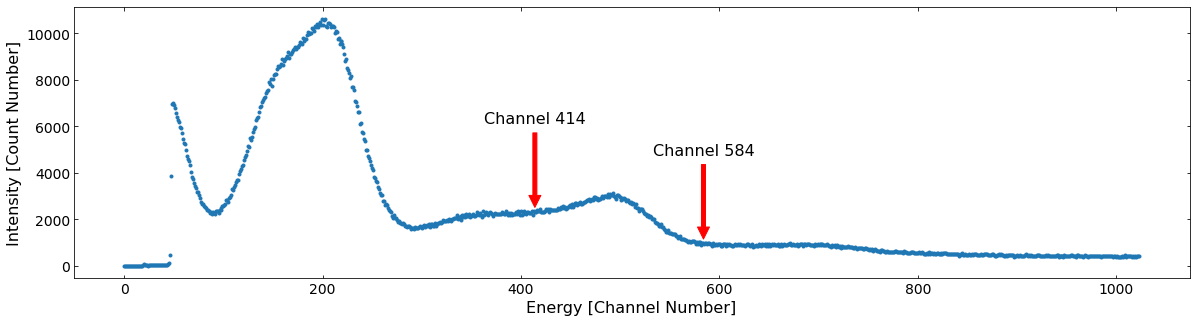
\includegraphics[width=1\columnwidth]{source_spectra_without_target.png}
        \caption{
                \label{fig:cospect} Energy discrimination range for the 14.4 KeV Co-57 gamma ray peak. The 1-$\sigma$ errorbar is too small to show on this plot.  
        }
\end{figure}    
    
    From (Fig.~\ref{fig:cospect}), we determined that the second peak is that of the 14.4 KeV emission. By setting the lower and upper level discriminators, the MCA was set to only receive pulses correlating to the desired energy spectrum.


\subsection{Mössbauer Mode}

    Once the MCA delimiters were set, the software was switched into Mössbauer mode. This mode allows for a dwell time to be set for each channel. Setting the dwell time to 200 us and the pass time on the CAD to 200 ms, each channel collected data for 200 us, corresponding to a small velocity range. The result of this collection is a set of counts that relates to an energy spectrum. Because each channel corresponds to a velocity range, the energy of the received photons can be calculated using Eqn~\ref{eqn:doppler}. 




\section{Raw Data}

Here is our raw data for absorption spectrum of Fe-57 (figure~\ref{fig:raw_data}).  Horizontal axis is scan time within an operation cycle, ranging from 0 to 200 ms, and recorded in 1024 channels. And we use calibration provided in the lab manual~\cite{labManual} to get our velocity axis. Each channel corresponds to a certain moving speed of gamma ray source, which can then be calibrated into energy shifts from stationary source (Eqn~\ref{eqn:doppler}). 
Vertical axis is intensity of penetrated radiation, less count number indicates higher absorption rate, with an 1-$\sigma$ error-bar. The background line is determined by averaging counts between the peaks (i.e. channels between 400 and 600), which indicates the noise level of our data. 

\begin{figure}[H] 
        \centering 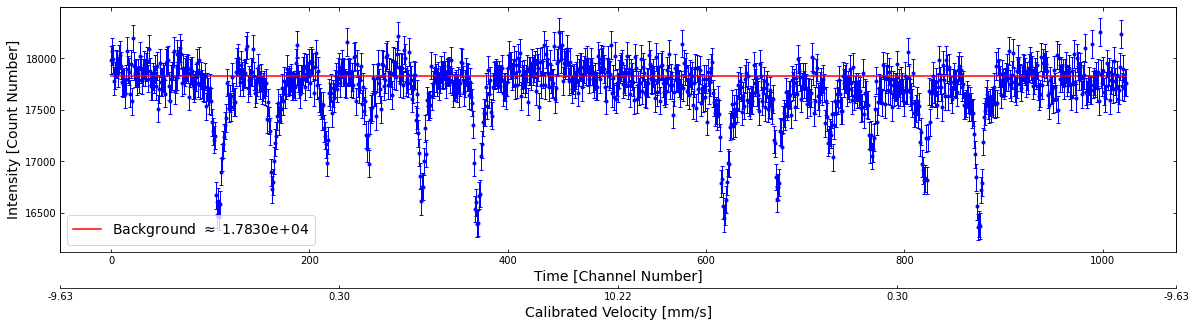
\includegraphics[width=1\columnwidth]{raw_data.png}
        \caption{\label{fig:raw_data}
        Absorption spectrum of Fe-57. 1-$\sigma$ error-bar represents counting standard deviation.
        }
\end{figure}

We get 12 absorption peaks being symmetric about the center channel. Each side represents the six allowed transitions between hyper-fine splitting states of ground and 1st excited state of Fe-57, which has been shown in Fig~\ref{fig:elevels}.  

\section{Results}
% \subsection{Gaussian Fit}
    
%     Here is a Gaussian fit of left part of our data (figure~\ref{fig:gauss_left}).
    
%     \begin{figure}[ht] 
%             \centering 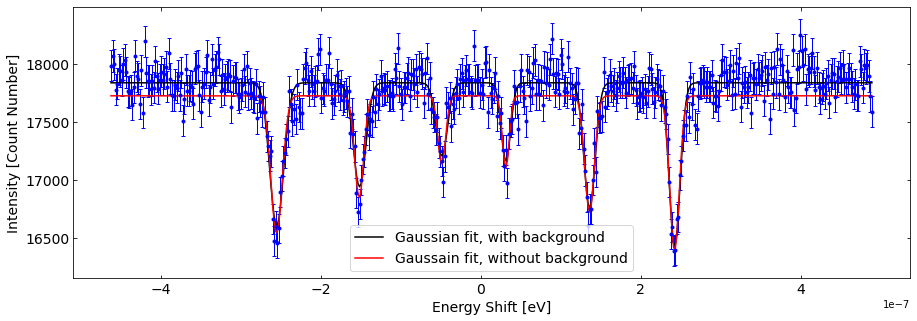
\includegraphics[width=1\columnwidth]{gauss_left.png}
%             \caption{
%                     \label{fig:gauss_left} From left to right, each peak (mean) represent an allowed transition between two hyper-fine splitting states, and the respective width (standard deviation) represents uncertainty in our measurement. 
%             }
    
%     \end{figure}
\subsection{Hyper-fine splitting spectrum}
    We calibrated velocity scale into energy scale using the Doppler effect (Eqn~\ref{eqn:doppler}), and fitted Lorentzian distribution to our absorption spectrum to study each peak (Fig~\ref{fig:lorentz_left}). As shown in Table~\ref{tbl:lorentz_fit}, energy spread around each peak is about one magnitude less than the mean value.

    
    \begin{figure}[ht] 
            \centering 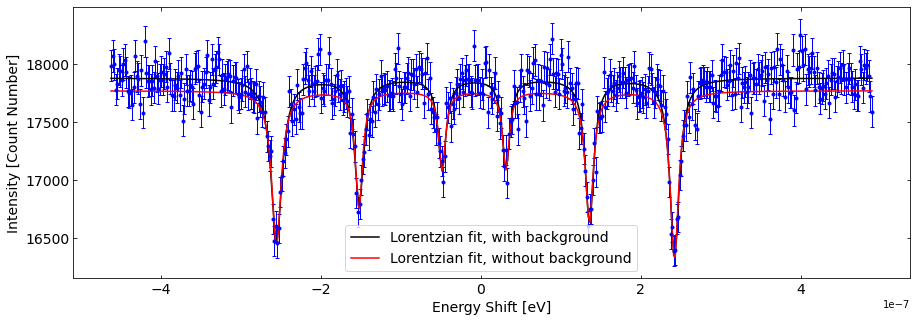
\includegraphics[width=1\columnwidth]{lorentz_left.png}
            \caption{
                    \label{fig:lorentz_left} Data fit to a linear combination of Lorentzian distributions about each peak%, using half-width as a measurement of uncertainty.
            }
    \end{figure}

\begin{table}[H]
\begin{center}
\caption{Peaks and associated energy shifts and linewidth.}
\label{tbl:lorentz_fit} % spaces are big no-no withing labels
\begin{tabular}{ccc}
\multicolumn{1}{c}{$\Delta E$ [$10^{-9}$ eV]} & \multicolumn{1}{c}{$\Gamma / 2$ [$10^{-9}$ eV]} & \multicolumn{1}{c}{Percent Error [$\%$]} \\
\hline
$-239.7$ & $10.56$ & 4.41\\
$-135.8$ & $9.75$ & 7.19\\
$-33.0$ & $8.45$ & 25.6\\
$46.1$ & $9.83$ & 21.3\\
$149.3$ & $9.34$ & 6.26\\
$253.5$ & $10.49$ & 4.14\\
\hline
\end{tabular}
\end{center}
\end{table}

These energies correspond to the shifts in transition energy due to hyper-fine splitting. (See Figure~\ref{fig:elevels}). Generally, the less the absorption is, the higher the effect of background noise will be. Error is higher for the inner peaks, which agrees with our figure(Fig~\ref{fig:lorentz_left}).  
% We also fitted the other half peaks. By comparing the mean value of the peaks, we found that there is an significant offset between them (Fig~\ref{fig:peak_compare}). We will discuss more on this in the Error Discussion section. 


\subsection{The bulk internal magnetic field}

These shifts in transition energy can be calculated by taking the difference between the split energy levels (Eqn.~\ref{eqn:split}) before and after the transition.

\begin{eqnarray}
        \Delta E = H\left(\frac{\mu_{\frac{1}{2}}m_{\frac{1}{2}}}{1/2} - \frac{\mu_{\frac{3}{2}}m_{\frac{3}{2}}}{3/2}\right) \label{eqn:transition}\,,
\end{eqnarray}

From the transitions between different first excited states (with different $m_{3/2}$) but the same ground state (with fixed $m_{1/2}$), we can get the difference between the energies of the excited state. From this, we can calculate the energy levels. Reference (Figure~\ref{fig:elevels}) for visual aid.

\begin{eqnarray}
        \Delta E_{m_1,m_2} = \Delta E_{m_2\rightarrow\pm\frac{1}{2}} - \Delta E_{m_1\rightarrow\pm\frac{1}{2}} = \frac{H\mu_{\frac{3}{2}}}{3/2}(m_1-m_2) \label{eqn:excitedE}\,,
\end{eqnarray}

For example, plugging into this equation $m_1$ = -1/2, $m_2$ = 1/2, and $m_{1/2}=-1/2$, we get $-1.017*10^{-7}$ eV $=-H\mu_{3/2}/(3/2)$. This is the difference in energy between the $m_{3/2}=\pm1/2$ states of the first excited state. We repeat this for the transition from $m_1=-3/2$ and $m_2=-1/2$ to $m_{1/2}=-1/2$ to get $-1.019*10^{-7}$ eV $=-H\mu_{3/2}/(3/2)$. This is the difference in energy between the $m_{3/2}=-3/2$ and $m_{3/2}=-1/2$ states.

We can also apply this procedure to transitions between the same excited state but different ground states to get the difference between the two energies of the ground state. Doing so with, say, the $m_{3/2}=-1/2$ state, we get $1.80*10^{-7}$ eV $=-H\mu_{1/2}/(1/2)$. The value for $\mu_{1/2}$ is $2.857*10^{-13}$ eV/G. Solving for H, we get H=314 kG. Because our calculations for this value involved only the difference in transition energies, the major uncertainty due to uncertainty in our starting velocity is not relevant. We can determine uncertainty in H using the following equation: 

\begin{eqnarray}
        \sigma_{\si{H}} = H\sqrt{\sum_{} \bigg(\frac{\sigma_{\si{E_{i,j}}}}{E_{\si{i,j}}}\bigg)^2}
        \label{eqn:erro_mag} \,,
\end{eqnarray}

The uncertainty in the energy is $\sqrt{2}$ times the error given by our least squares fit \rightarrow{} $\pm8*10^{-10}$ and the uncertainty in $\mu_{1/2}$ is 0.00007 nm $=2*10^{-16}$ eV/G (given). Plugging into Equation ~\ref{eqn:erro_mag}, we get an uncertainty of $\pm3$ kG.

% We calculated the internal magnetic field to be $2.990(\pm 0.036) \times 10^5$ G
%    Mean [eV]    Half-Width [eV]    Magnetic Field [G]
% ------------  -----------------  ------------------------
%  2.64775e-07        1.5381e-08                     322082
%  1.62716e-07        1.31392e-08                    325777
%  6.07592e-08        1.57232e-08                    344631
% -1.7497e-08         1.15005e-08                    223419
% -1.19346e-07        1.32831e-08                    290729
% -2.23839e-07        1.25725e-08                    305243

\subsection{The magnetic moment of the first excited state}

Now that we know H, all we have to do is plug this into equation~\ref{eqn:excitedE}. Calculating for error in the same way as for H using Equation~\ref{eqn:erro_mag}, this gives $(4.86\pm0.05)*10^{-13}$ eV/G.


\subsection{Error Discussion}
    
    The biggest source of error arose from our low confidence in the calibration information provided in our lab manual ~\cite{labManual}. As shown in Figure~\ref{fig:peak_compare}, the offset between two sides exceeds the error bar, which cannot be explained by energy spreading or uncertainty principle. So we shifted our data by calculating average of peak and its symmetric counterpart (Fig~\ref{fig:peak_compare}). 
    \begin{figure}[ht] 
            \centering 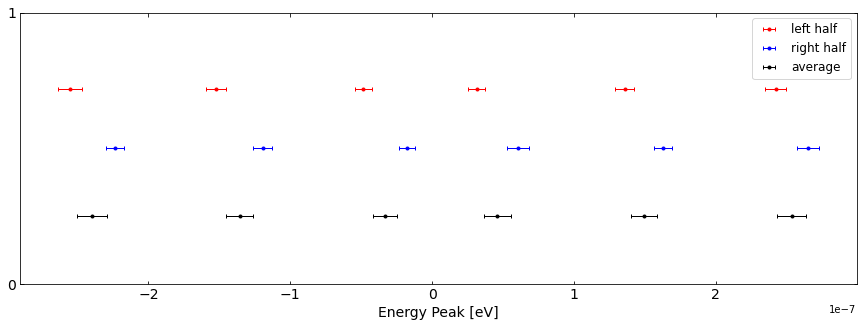
\includegraphics[width=1\columnwidth]{peak_compare.png}
            \caption{
                    \label{fig:peak_compare} Peak found using Lorentzian fit, with error bar defined as half of the linewidth $\frac{\Gamma}{2}$. Absorption peaks for the right half are generally shifted to the right, which may be resulted from systematic error.
            }
    \end{figure}

    % The information provided is inconsistent with our data.   (Figure~\ref{fig:longplot})
    
    % \begin{figure}[ht] 
    %         \centering 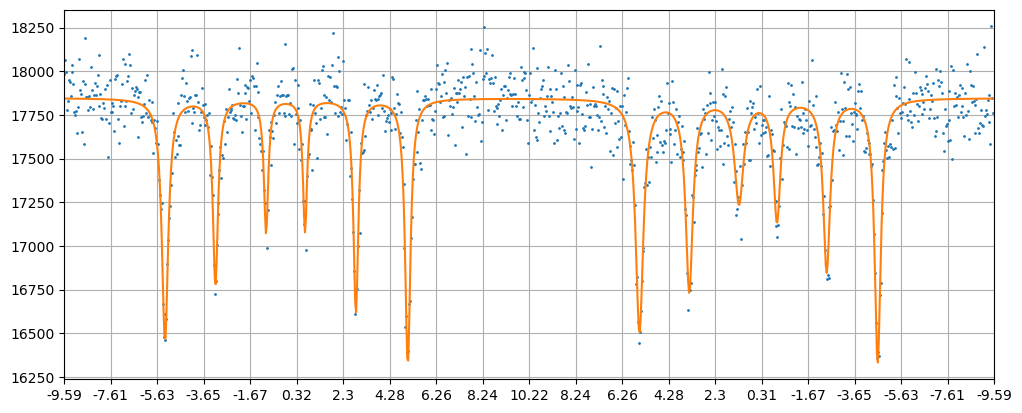
\includegraphics[scale=0.6]{longplot.png}
    %         \caption{
    %                 \label{fig:longplot}
    %                 Plot with width expanded to see symmetry of data
    %         }
    % \end{figure}
    
    The lab manual provides the following information: channel 0 measures the lowest velocity -9.59 mm/s. The CAD goes from -9.59 mm/s to 10.22 mm/s and back in 200 ms (with constant acceleration). Each channel operates for 0.2 ms. From this, we can deduce that channel 500 measures the 10.22 mm/s velocity, and channel 1000 measures -9.59 mm/s. As the CAD ranges through the velocities about either side of the maximum at channel 500, the absorption peaks should also be symmetric about this point.
    
    It is not, however, and we do not know the source and content of the error. We assume that the 0.2 ms dwell time of each channel is accurate. Assuming that the provided minimum and maximum values of the velocity are accurate, there are two possibilities to explain the inconsistency. 
    
    (1) The period of the cycle of the CAD is less than 200 ms.
    
    (2) The minimum velocity does not coincide with channel 0. The velocity at channel 0 is a little more than -9.59s.
    
    For our calculations, we assume the second possibility, not for any profound reason, but that it seems to be the simpler explanation. In line with this assumption, we defined the maximum velocity to be located at the midpoint between the two sets of peaks. We also assume that the provided minimum and maximum velocity values are accurate, although we have as much reason to trust them as we know that parts of the other information provided with them are wrong.

    The midpoint is at channel 492, different from the theoretical 500 by 8 channels, 0.3 mm/s, or $2*10^{-8}$ eV. We took this to mean that there is a general uncertainty in the experimental process of at least this amount. This is in addition to the error of our energies (channels) given by the least squares fitting of 0.3 channels or 0.01 mm/s or $6*10^{-10}$ eV




\section{Discussion}

We conclude that the magnetic moment of the first excited state of Fe-57 is $\mu_{3/2}=4.86*10^{-13}$ with an error of $\pm5*10^{-15}$. As we compare this to the accepted value of $\mu_{3/2}=-4.896e-13$ eV/G, we see that our conclusion and error estimates fall within the range of our derived value and error.


We conclude that the size of the magnetic field for Fe-57 is 314 kG with an error of 3 kG.



%++++++++++++++++++++++++++++++++++++++++


\begin{thebibliography}{99}

\bibitem{labManual}
UCSB Physics Department. (2018). The Mossbauer Effect. \texttt{http://web.physics.ucsb.edu/~phys128/experiments/interferometry/Precision-Interferometer-Manual-OS-9255A.pdf}

\bibitem{lorentz}
Cauchy distribution. Wikipedia. Retrieved February 3, 2023, from 
\texttt{https://en.wikipedia.org/wiki/Cauchy_distribution}.

\end{thebibliography}




\end{document}




\ref{fig:name}


\begin{figure}[ht] 
        % read manual to see what [ht] means and for other possible options
        \centering \includegraphics[width=1\columnwidth]{sr_setup}
        % note that in above figure file name, "sr_setup",
        % the file extension is missing. LaTeX is smart enough to find
        % apropriate one (i.e. pdf, png, etc.)
        % You can add this extention yourself as it seen below
        % both notations are correct but above has more flexibility
        %\includegraphics[width=1.0\columnwidth]{sr_setup.pdf}
        \caption{
                \label{fig:samplesetup} % spaces are big no-no withing labels
                % things like fig: are optional in the label but it helps
                % to orient yourself when you have multiple figures,
                % equations and tables
                Every figure MUST have a caption.
        }
\end{figure}


\begin{table}[ht]
\begin{center}
\caption{Every table needs a caption.}
\label{tbl:bins} % spaces are big no-no withing labels
\begin{tabular}{|cc|} 
\hline
\multicolumn{1}{|c}{$x$ (m)} & \multicolumn{1}{c|}{$V$ (V)} \\
\hline
0.0044151 &   0.0030871 \\
0.0021633 &   0.0021343 \\
0.0003600 &   0.0018642 \\
0.0023831 &   0.0013287 \\
\hline
\end{tabular}
\end{center}
\end{table}


\begin{acknowledgments}
Thanks to Dr. Jayich for guidance of this lab and editing of this report.
\end{acknowledgments}
